\documentclass[a4,12pt]{scrartcl}

%Basic 
\usepackage[utf8]{inputenc}
\usepackage[ngerman]{babel}
\usepackage[T1]{fontenc}
\usepackage{float}
%\usepackage[bottom = 3.50cm]{geometry}

%Titel Seite
\title{CLOUD INFRASTRUCTURE}
\subtitle{Lab-04}
\author{Giorgio Vincenti und Samuel Krieg}
\date{\today}


%Kopf, Fusszeile
\usepackage{fancyhdr}
\pagestyle{fancy}
\lhead{ \begin{picture}(0,0) \put(0,0){
\includegraphics[width=3cm]{./pictures/hsrlogo.png}} \end{picture}}
\chead{}
\rhead{Seite \thepage}
\lfoot{Cloud Infrastructure \\Lab-04}
\cfoot{Giorgio Vincenti und Samuel Krieg}
\rfoot{\today}
\renewcommand{\headrulewidth}{0.4pt}

%Bilder
\usepackage{graphicx}
\usepackage{wrapfig}

%Tabellen
\usepackage{booktabs}

%Codesnippets
\usepackage{listings}
\lstset{language=bash}  

%Querformat für eine Seite
\usepackage{lscape}
\usepackage{rotating}
\usepackage{pdflscape}

%Temp
\usepackage{lipsum}



\begin{document}

\clearpage\maketitle
\thispagestyle{empty}
\tableofcontents

\section{Aufgabenstellung}
Wurde aus der Aufgabenstellung entnommen:

\noindent Your teammate needs your help. She works in the software development team and is not really experienced in Linux server and virtualization. Create a How-to for your workmate in order that the software developer can use it.

\noindent \textbf{What they need:}
\begin{itemize}
\item 3 separated virtual machines
\item  VM1 has to be reachable from the internet and needs connectivity to VM2
\item VM2 needs connectivity to VM3
\item It has to be runnable on a virtual Linux server without GUI
\item Guess how long it will take for the SE
\end{itemize}

\textbf{Add the following to your delivery:}
\begin{itemize}
\item Usability
\item Is it possible to deploy the VMs on multiple hosts (2 Nodes)?
\end{itemize}

\textbf{Hints}
\begin{itemize}
\item Download Qcow image for VM
\item Qemu supports different network backend types
\item Guest VM don’t need a GUI
\end{itemize}


\subsection{Wichtiges im Überblick}
Hier einen Überblick über die erforderlichen Punkte:
\begin{itemize}
\item Anleitung für Software Engineering 
\begin{itemize}
\item Anleitung für erstellen / verwalten von VMs
\end{itemize}
\item 3 virtuelle Maschinen installieren
\item VM1 muss vom Internet aus erreichbar sein
\item VM2 muss mit VM3 kommunizieren können
\item Dauer einer Installation abschätzen / messen
\item Verwendbarkeit aufzeigen
\item Einsatz der VMs auf mehreren Hosts abklären
\end{itemize}

\subsection{Kriterien}
Wurden aus dem Mail von Urs Baumann entnommen: 
\begin{itemize}
\item Struktur
\item Verständlich für Software Entwickler
\item Funktionalität 
\item Kapitel zu Usability 
\item Eingesetzte Netzwerktypen 
\item Kapitel zu "multi host setup"  
\end{itemize}
\newpage

\section{Infrastruktur}
Hier einige Eckdaten zu der Infrastruktur. 

\subsection{Virtualisierungs-Software (Test-Umgebung)}
Um die Aufgabe durchzuführen wird die erforderliche Umgebung auf VMWare Workstation 12.0 aufgesetzt. 

\subsection{Virtualisierungs-Host}
Als Virtualisierungs-Host wir ein Linux OS eingsetzt. Wir gehen nicht auf die Details der Installation ein. Es wird nur das nötigste dokumentiert.  

\subsubsection{OS} 
Hier einige Details über die eingesetzte Linux Distribution. 
\begin{center}
    \begin{tabular}{@{} l l r@{}}\toprule    
    {Linux Distribution} & {Version}\\ \midrule
    Ubuntu & 14.04.3 LTS\\ \addlinespace
    \bottomrule
    \end{tabular}
\end{center}

\subsubsection{Login}
Um VMs auf dem Host erstellen zu können sind Berechtigungen erforderlich. Die Userin wird auf dem Host-Computer mit einem Administratorkonto arbeiten. 
\begin{center}
    \begin{tabular}{@{} l l r@{}}\toprule    
    {Benutzername} & {Passwort} & {Privilegien}\\ \midrule
    Cloud Infrastrucure & hsr12344 & Administrator (root)\\ \addlinespace
    \bottomrule
    \end{tabular}
\end{center}

\subsubsection{Network}
Der Host verfügt über eine statische IP-Konfiguration. Die Netzwerkkarte wird in der VMWare Workstation im NAT-Modus betrieben, um Internetkonektitivät zu erhalten.  
\begin{center}
    \begin{tabular}{@{} l l r@{}}\toprule    
    {Hostname} & {IP-Adresse} & {Subnetz}\\ \midrule
    Host & 10.0.0.101 & 255.255.255.0\\ \addlinespace
    \bottomrule
    \end{tabular}
\end{center}
Auf dem VMWare Virtual Network ist ein DHCP Service aktiviert. \\
Subnet: 10.0.0.0 und Netmask: 255.255.255.0 \\
DHCP-Pool: 10.0.0.150 - 10.0.0.180

\subsubsection{Services}
Auf dem Server laufen keine, für die Umgebung relevanten, Services. Es sind die Standard-Features von Ubuntu installiert.  

\subsubsection{Application}
Auf dem Ubuntu Client (Host) wird als Virtualisierungssoftware QEMU eingesetzt. Mit dieser Software soll die Anwenderin VMs erstellen und verwalten können. 
\begin{center}
    \begin{tabular}{@{} l l r@{}}\toprule    
    {Software} & {Version}\\ \midrule
    QEMU emulator & 2.0.0\\ \addlinespace
    \bottomrule
    \end{tabular}
\end{center}
Die Installation der Software erfolgte über das Terminal: 
\begin{center}
    \begin{tabular}{@{} l l r@{}}\toprule    
    {Befehl} & {Bemerkung}\\ \midrule
    apt-get install qemu-system & Download und Installation\\
     \addlinespace
    \bottomrule
    \end{tabular}
\end{center}

\subsection{Virtualisierungs-Guests}
Die Umgebung besteht aus gesamt drei virtuellen Guests, die auf dem Virtualisierungs-Host laufen. Als Virtualisierungssoftware wird QEMU eingesetzt. 

\subsubsection{Guest-OS}
Als Guest-OS wird auf eine extrem kleine Linux Distribution gesetzt. Alle drei VMs betreiben dasselbe OS. 
\begin{center}
    \begin{tabular}{@{} l l r@{}}\toprule    
    {Distribution} & {Version} & {Hostname}\\ \toprule
    Tiny Core & v6.4 & vm1guest\\ 
    Tiny Core & v6.4 & vm2guest\\
    Tiny Core & v6.4 & vm3guest\\ \addlinespace
    \bottomrule
    \end{tabular}
\end{center}

\subsubsection{Guest-Path}
Die VMs befinden sich im Homeverzeichnis des Users. Sie sind als *.img Datei abgelegt.
\begin{center}
    \begin{tabular}{@{} l l r@{}}\toprule    
    {Image-Name} & {Path} & {Hostname}\\ \toprule
    vm1\_guest.img & /home/cldinf/Virtualdir & vm1guest\\ 
    vm2\_guest.img & /home/cldinf/Virtualdir & vm2guest\\
    vm3\_guest.img & /home/cldinf/Virtualdir & vm3guest\\ \addlinespace
    \bottomrule
    \end{tabular}
\end{center}

\begin{figure} [H]
	\begin{center}
	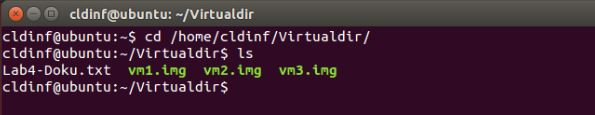
\includegraphics[width=0.80\textwidth]{./pictures/virtualdir.jpg}
	\caption{{Virtualdir Übersicht}}
	\label{virtualdir}
	\end{center}
\end{figure}

\subsubsection{Guest-Networking}
Hier einige Details über die IP-Konfiguration der Guests. Jeder Guest verfügt über zwei Schnittstellen.  
\begin{center}
    \begin{tabular}{@{} l l r@{}}\toprule    
    {Hostname} & {IP-Adresse} & {Netmask}\\ \toprule
    vm1guest & 10.10.0.11 + 1.11 & 255.255.255.0\\ 
    vm2guest & 10.10.1.12 + 2.11 & 255.255.255.0\\
    vm3guest & 10.10.2.12 & 255.255.255.0\\ \addlinespace
    \bottomrule
    \end{tabular}
\end{center}

\subsection{Networking}
In diesem Kapitel werden einige Konfigurationsdetails zum Netzwerk aufgezeigt.
\begin{figure} [H]
	\begin{center}
	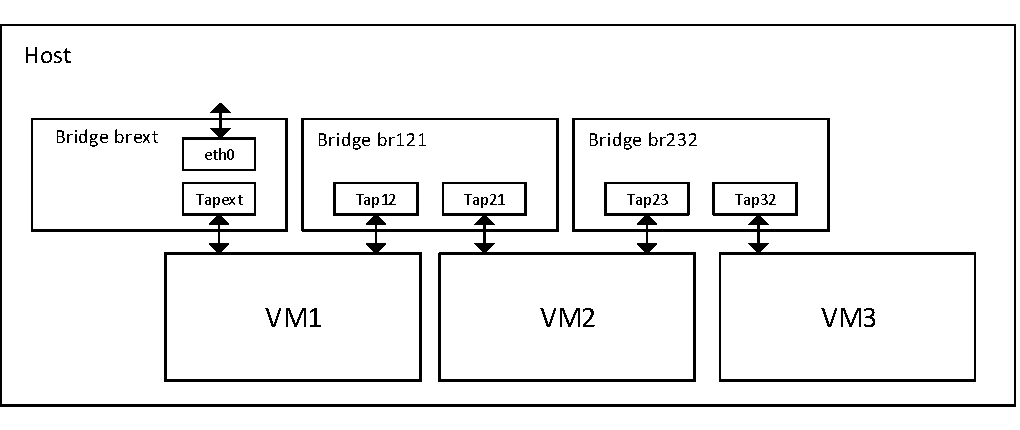
\includegraphics[width=0.80\textwidth]{./draws/uebersicht_bridges_taps_visio.pdf}
	\caption{{network overview}}
	\label{virtualdir}
	\end{center}
\end{figure}

\noindent Zur Sicherstellung der Kommunikationswege werden die Layer 2 Verbindungen über Bridges realisiert. Die Guest-OS werden mittels TAP's in die Birdges eingebunden. Damit VM1 mit dem Netzwerk kommunizieren kann, muss eine Bridge konfiguriert werden welche das Netwerkinterface  des Host-OS beinhaltet.

\subsubsection{Host-Networkconfig}
Wurde bereits im obigem Kapitel aufgelistet. (Kapitel 2.2.3)
 
\subsubsection{Bridge}
Es sind gesamt drei Bridges notwendig um die Umgebung zu betreiben. Zwei Bridges zwischen den VM's und eine für die Kommunikation  nach aussen.
\begin{center}
    \begin{tabular}{@{} l l r@{}}\toprule    
    {Bridge Name} & {Verbindung} & {Intfaces}\\ \toprule
    brext & HostOS-VM1 & eth0,tapext\\ 
    br121 & VM1-VM2 & tap12,tap21\\
    br323 & VM2-VM3 & tap23,tap32\\ \addlinespace
    \bottomrule
    \end{tabular}
\end{center}
\subsubsection{Guest-Networkconfig}
Wurde bereits im obigen Kapitel aufgelistet. (Kapitel 2.3.3)\\
In der Anleitung mehr Details dazu. 

\section{Anleitung}
Dies ist eine kurze Anleitung für das erstellen einer 3-Tier Umgebung mit \textbf{QEMU} auf einer Linux-Umgebung. Es wird von Ubuntu 14.04 als Hosts-OS ausgegangen.

\subsection{Was benötigt wird}
Um die Umgebung aufzubauen wird folgendes benötigt: 
\begin{itemize}
\item Ein Host-OS um \textbf{QEMU} betreiben zu können
\item \textbf{QEMU} Software auf dem Host-OS 
\item Ein Guest-OS, welche die 3-Tier Umgebung darstellen 
\item Diverse Netzwerk-Konfigurationen seitens des Host 
\end{itemize}

\subsection{Vorgehen}
Wir gehen bereits davon aus das die Userin ein Host-OS installiert hat.
Die Vorbereitungen sind im Terminal auf dem Host-OS vorzunehmen. 

\subsubsection{Installation und Vorbereitung}
\begin{itemize}
\item Installation der Virtualisierungssoftware \textbf{QEMU}:
\begin{lstlisting} 
sudo apt-get install qemu
\end{lstlisting}
\item Installation des Packets \textbf{bridge-utils} für das Bridgemanagement:
\begin{lstlisting}
sudo apt-get install bridge-utils
\end{lstlisting}
\end{itemize} 

\begin{itemize}
\item Erweitere Zugriffsrechte auf das \textbf{TUN-Device} für group und others erteilen:
\begin{lstlisting}
sudo chmod go+rw /dev/net/tun
\end{lstlisting}
\end{itemize}

\begin{itemize}
\item Anpassen der \textbf{QEMU} Interface up \& down Skripte:
\newline
Jeweils die Inhalte ersetzen (mit root-Rechte anpassen):
\newline
/etc/qemu-ifup:
\begin{lstlisting}
#!/bin/sh                                                        
sudo -p /sbin/ifconfig $1 0.0.0.0 up
\end{lstlisting}
/etc/qemu-ifdown:
\begin{lstlisting}
#!/bin/sh                                                        
sudo -p /sbin/ifconfig $1 down
\end{lstlisting}
\end{itemize}
Die Dateien liegen ebenfalls im Virtualdir/settings Verzeichnis, falls die Userin lieber die Dateien ersetzen möchte, statt diese zu bearbeiten. 

\begin{itemize}
\item Sofern \textbf{qemu-ifup} \& \textbf{qemu-ifdown} nicht bereits ausführbar sind, dies nachholen:
\begin{lstlisting}
sudo chmod +x /etc/qemu-ifup
sudo chmod +x /etc/qemu-ifdown
\end{lstlisting}
\end{itemize}

\subsubsection{Guest-OS}
Die Guest-OS liegen als Images (*.img) im home Verzeichnis des Users unter Virtualdir. 
\begin{itemize}
\item Starten der VM's mittels QEMU und erzeugen der \textbf{TAP}'s:
\begin{lstlisting}
sudo qemu-system-x86_64 Virtualdir/vm1_guest.img -nographic 
-net nic, -net tap,ifname=tapext -net nic, -net tap,ifname=tap12

sudo qemu-system-x86_64 Virtualdir/vm2_guest.img -nographic
-net nic, -net tap,ifname=tap21 -net nic, -net tap,ifname=tap23

sudo qemu-system-x86_64 Virtualdir/vm3_guest.img -nographic
-net nic, -net tap,ifname=tap32
\end{lstlisting}
Die TAP's und Bridges sollten nun bei der Eingabe von \textit{ifconfig} auf dem Host-OS ersichtlich sein.

\item In den Guest-OS müssen den Netzwerkinterfaces IP-Adressen zugewiesen werden. Die folgenden Befehlesind in den Guest-OS auszuführen.
\newline
VM1:
\begin{lstlisting}
sudo ifconfig eth0 10.10.0.11 netmask 255.255.255.0 up
sudo ifconfig eth1 10.10.1.11 netmask 255.255.255.0 up
\end{lstlisting}
VM2:
\begin{lstlisting}
sudo ifconfig eth0 10.10.1.12 netmask 255.255.255.0 up
sudo ifconfig eth1 10.10.2.11 netmask 255.255.255.0 up
\end{lstlisting}
VM3:
\begin{lstlisting}
sudo ifconfig eth1 10.10.2.12 netmask 255.255.255.0 up
\end{lstlisting}
\end{itemize}

\subsubsection{Bridges}
Die Bridges werden auf dem Host-OS erstellt. Insgesamt werden drei Bridges benötigt. 
\begin{itemize}
\item Erstellen der \textbf{Bridges}:
\begin{lstlisting}
sudo brctl addbr brext
sudo brctl addbr br121
sudo brctl addbr br323
\end{lstlisting}

\item Die durch das starten der VM's erstellten TAPS müssen nun den Bridges zugeordnet werden:
\newline

Bridge \textbf{brext}:
\begin{lstlisting}
sudo brctl addif brext eth0
sudo brctl addif brext tapext
\end{lstlisting}

Bridge \textbf{br121}:
\begin{lstlisting}
sudo brctl addif br121 tap12
sudo brctl addif br121 tap21
\end{lstlisting}

Bridge \textbf{br323}:
\begin{lstlisting}
sudo brctl addif br323 tap23
sudo brctl addif br323 tap32
\end{lstlisting}


\item Den Bridges die \textbf{IP's zuweisen}:
\begin{lstlisting}
sudo ifconfig brext 10.10.0.1 netmask 255.255.255.0 up
sudo ifconfig br121 10.10.1.1 netmask 255.255.255.0 up
sudo ifconfig br323 10.10.2.1 netmask 255.255.255.0 up
\end{lstlisting}
\end{itemize}
Als Abschluss kann die komplette Konektivität mittels Ping-Befehle getestet werden. Nun sollte die Umgebung funktionieren. 
\newpage

\section{Testing}
Mit einigen Pings können Tests durchgeführt werden. Hier folgen einige Test-Beispiele. 

\subsection{VM1 to Internet}
\begin{figure} [H]
	\begin{center}
	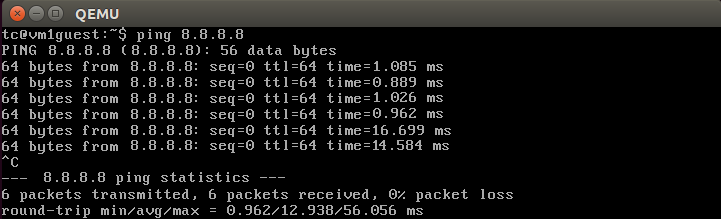
\includegraphics[width=0.80\textwidth]{./pictures/ping_vm1_to_internet.png}
	\caption{{Ping test von VM1 ins Internet (Google Public DNS)}}
	\label{virtualdir}
	\end{center}
\end{figure}

\subsection{VM1 to VM2}
\begin{figure} [H]
	\begin{center}
	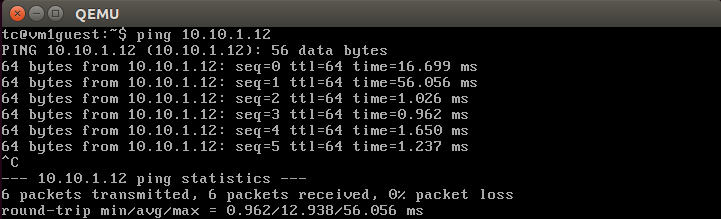
\includegraphics[width=0.80\textwidth]{./pictures/ping_vm1_to_vm2.png}
	\caption{{Ping test von VM1 zu VM2}}
	\label{virtualdir}
	\end{center}
\end{figure}

\subsection{VM2 to VM3}
\begin{figure} [H]
	\begin{center}
	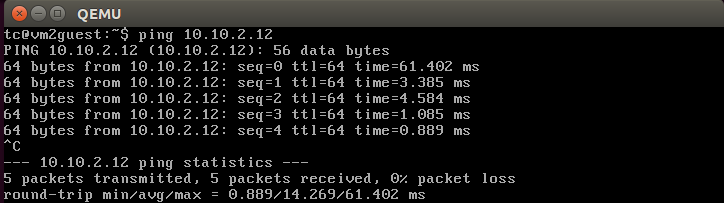
\includegraphics[width=0.80\textwidth]{./pictures/ping_vm2_to_vm3.png}
	\caption{{Ping test von VM2 zu VM3}}
	\label{virtualdir}
	\end{center}
\end{figure}
\newpage

\section{Usability}
Es ist definitiv zumutbar für einen Softwareentwickler. Es werden drei Scripte vorbereitet, welche all diese Schritte automatisieren. Das erste Script(Vorbereitung.sh) benötigt etwas länger zum durchlaufen wegen den Installationen der Module. Die Zeit hängt von der Leistungsfähigkeit des Computers,der Internetanbindung und der Grösse des Guest-Image ab. Nach dem Setup kann mit Ausführzeiten der zwei weiteren Scripts(StartenDerVMs.sh \& NetworkSettings.sh) kleiner 1min gerechnet werden. 

\section{3-Tier Modell auf anderen Host}
Die Frage ist jetzt, ob das 3-Tier Modell auf einem beliebigem (oder einen anderen Host) gemäss dieser Anleitung betrieben werden kann. 

\noindent Natürlich kann die Umgebung auf einem anderen Host betrieben werden. Um das Host-OS zu wechseln muss die Userin nur drei Scripts ausführen die wir in ihr Home Verzeichnis gepackt haben. Zusätzlich müssen die Images der Guest-OS auf dem anderen Host kopiert werden oder Home Verzeichnis Roaming muss aktiviert sein (falls bsp.: Active Directory vorhanden). Falls kein Romaing aktiv ist, wäre das einfachste das Verzeichnis Virtualdir auf den anderen Host zu kopieren. Die VM-Guest Netzwerk Einstellungen sind manuell durchzuführen. 

\subsection{Virtualdir}
Hier der Inhalt des Verzeichnis Virtualdir im Home Verzeichnis. 
\begin{itemize}
\item /home/cldinf/Virtualdir/scripts/Vorbereitung.sh
\item /home/cldinf/Virtualdir/scripts/StartenDerVMs.sh 
\item /home/cldinf/Virtualdir/scripts/NetworkSettings.sh
\item /home/cldinf/Virtualdir/vm1\_guest.img
\item /home/cldinf/Virtualdir/vm2\_guest.img
\item /home/cldinf/Virtualdir/vm3\_guest.img 
\item /home/cldinf/Virtualdir/settings/qemu-ifup
\item /home/cldinf/Virtualdir/settings/qemu-ifdown
\end{itemize}
\end{document}
